\chapter{Stereochemistry: Chirality and Isomers}\label{ch:g12:stereochemistry}

Spearmint leaves and caraway seeds smell nothing alike: one is the fresh
smell of chewing gum, the other the warm smell of rye bread. Yet the
\omterm{def:g7:atoms-and-molecules:molecule}{molecule} responsible for each smell is the same carvone, made of the same
\omterm{def:g7:atoms-and-molecules:atom}{atoms} bonded in the same order. The two carvones differ only as a left
hand differs from a right hand: each is the mirror image of the other.
Our nose, built of \omterm{def:g7:atoms-and-molecules:molecule}{molecules} that are themselves ``handed'', tells them
apart. This chapter learns to see \omterm{def:g7:atoms-and-molecules:molecule}{molecules} in three dimensions.

\begin{recall}
The shape of \omterm{def:g7:atoms-and-molecules:molecule}{molecules}, and the wedges and dashes that draw them in
space (\cref{ch:g10:lewis-and-shape}). \omterm{def:g11:organic-skeletons:isomer}{Constitutional isomers}
(\cref{ch:g11:organic-skeletons}). \omterm{def:g11:functional-groups:functional-group}{Functional groups}
(\cref{ch:g11:functional-groups}).
\end{recall}

\begin{omfigure}
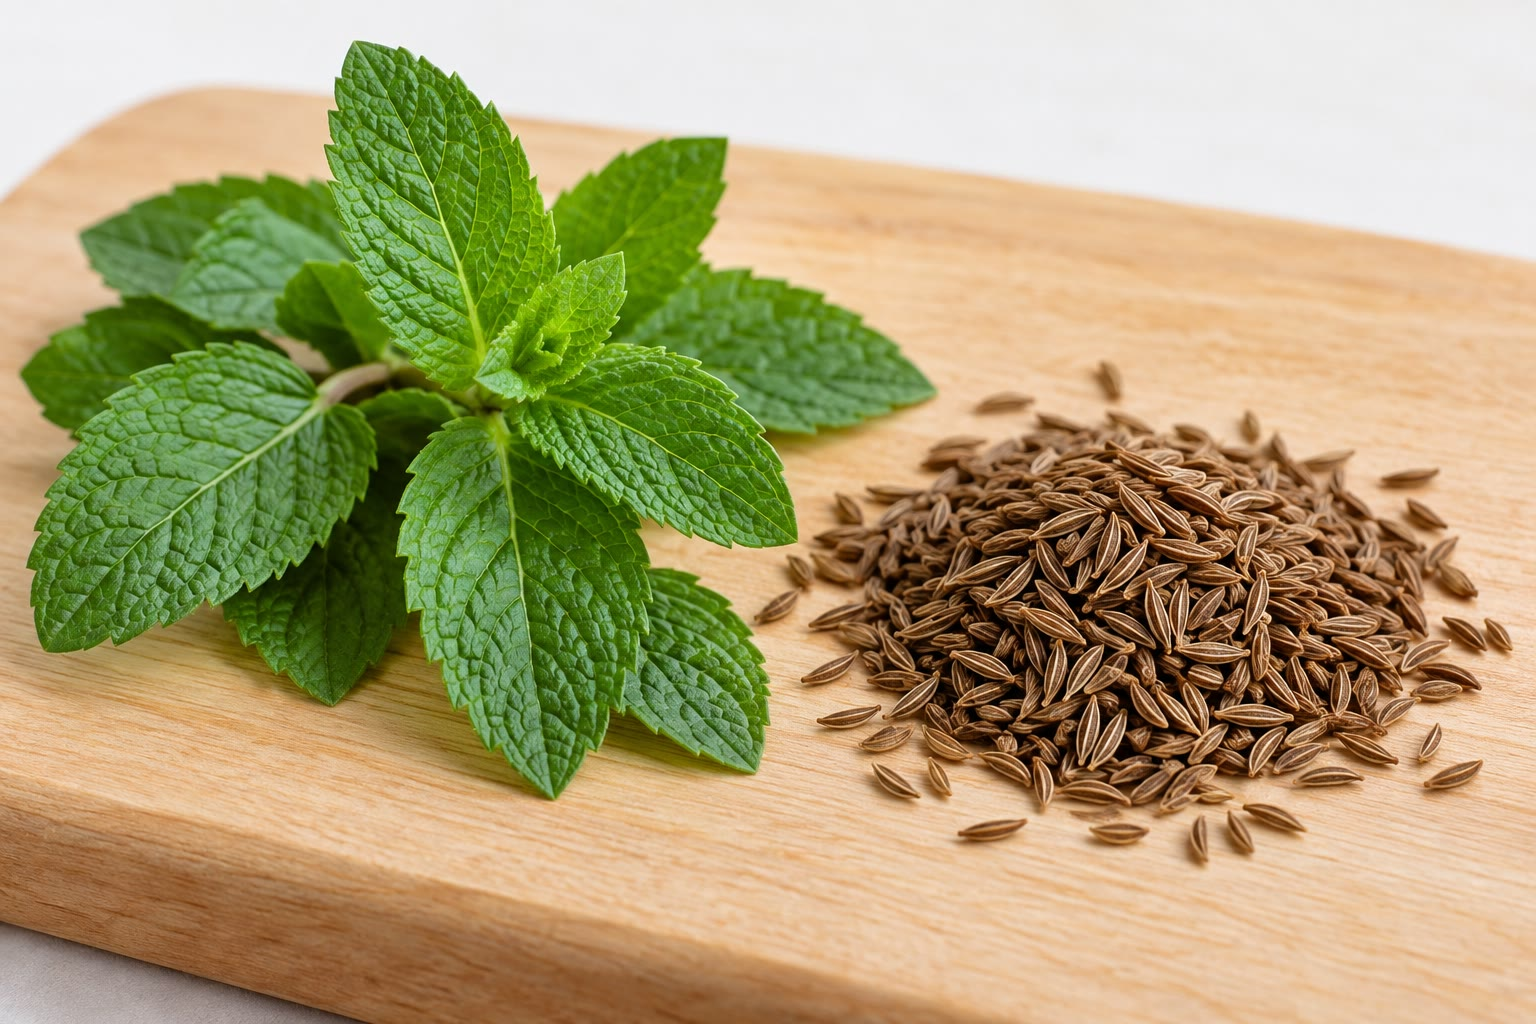
\includegraphics[width=0.48\linewidth]{images/book1/ai/g12-mint-caraway.jpg}

{\small Spearmint and caraway: two mirror-image \omterm{def:g7:atoms-and-molecules:molecule}{molecules}, two smells.}
\end{omfigure}

\section{Molecules in space}

\begin{definition}[Stereoisomers]\label{def:g12:stereochemistry:stereoisomer}
\emph{Stereoisomers}\index{stereoisomers} are \omterm{def:g7:atoms-and-molecules:molecule}{molecules} with the same
formula and the same sequence of bonded \omterm{def:g7:atoms-and-molecules:atom}{atoms}, which differ only by the
arrangement of their \omterm{def:g7:atoms-and-molecules:atom}{atoms} in space.
\end{definition}

\begin{definition}[Cram representation]\label{def:g12:stereochemistry:cram}
In the \emph{Cram representation}\index{Cram representation} of a carbon
\omterm{def:g7:atoms-and-molecules:atom}{atom} with four single bonds, two bonds are drawn in the plane of the
paper as plain lines, at an angle, the bond pointing towards the reader
as a solid wedge and the bond pointing away as a dashed wedge.
\end{definition}

\section{Chirality}

\begin{definition}[Chiral, asymmetric carbon]\label{def:g12:stereochemistry:chiral}
An object or a \omterm{def:g7:atoms-and-molecules:molecule}{molecule} is \emph{chiral}\index{chiral} if it cannot be
superimposed on its mirror image, like a hand. A carbon \omterm{def:g7:atoms-and-molecules:atom}{atom} bonded to
four different \omterm{def:g7:atoms-and-molecules:atom}{atoms} or groups is an \emph{asymmetric
carbon}\index{asymmetric carbon}; it is often marked with a star.
\end{definition}

\begin{proposition}[One asymmetric carbon makes a molecule chiral]\label{prop:g12:stereochemistry:one-carbon}
A \omterm{def:g7:atoms-and-molecules:molecule}{molecule} with exactly one \omterm{def:g12:stereochemistry:chiral}{asymmetric carbon} is \omterm{def:g12:stereochemistry:chiral}{chiral}.
\end{proposition}

\begin{proof}
Admitted: exchanging two of the four different groups around the
\omterm{def:g12:stereochemistry:chiral}{asymmetric carbon} gives the mirror image, and no rotation of the whole
\omterm{def:g7:atoms-and-molecules:molecule}{molecule} can bring it back, since the four groups are all different.
\end{proof}

\begin{definition}[Enantiomers, racemic mixture]\label{def:g12:stereochemistry:enantiomer}
Two \omterm{def:g12:stereochemistry:stereoisomer}{stereoisomers} that are mirror images of each other and not
superimposable are \emph{enantiomers}\index{enantiomers}. A \omterm{def:g6:pure-substances-and-mixtures:mixture}{mixture} of
equal amounts of two enantiomers is a \emph{racemic
mixture}\index{racemic mixture}.
\end{definition}

\begin{omfigure}
\setchemfig{atom sep=2.2em}
\begin{tikzpicture}[font=\small]
  \node at (-2.4,0) {\chemfig{C(-[2]COOH)(-[4]H_3C)(<[:-30]OH)(<:[:-150]H)}};
  \node at (2.4,0) {\chemfig{C(-[2]COOH)(-[0]CH_3)(<[:-150]HO)(<:[:-30]H)}};
  \draw[dashed, omDef, thick] (0,-1.5) -- (0,1.6) node[above] {mirror};
  \node[anchor=north] at (-2.4,-1.4) {lactic acid, A};
  \node[anchor=north] at (2.4,-1.4) {its mirror image, B};
\end{tikzpicture}

{\small The two \omterm{def:g12:stereochemistry:enantiomer}{enantiomers} of lactic acid, \ce{CH3-CH(OH)-COOH}, in \omterm{def:g12:stereochemistry:cram}{Cram
representation}. The central carbon is asymmetric (\ce{H}, \ce{OH},
\ce{CH3}, \ce{COOH}). No rotation turns A into B: they are as different
as a left and a right hand.}
\end{omfigure}

\begin{method}[Is a molecule chiral?]\label{met:g12:stereochemistry:chiral}
\begin{enumerate}
  \item Look for \omterm{def:g12:stereochemistry:chiral}{asymmetric carbons}: a carbon with four different
        groups. None: the \omterm{def:g7:atoms-and-molecules:molecule}{molecule} is (in this book) not \omterm{def:g12:stereochemistry:chiral}{chiral}.
  \item Exactly one: the \omterm{def:g7:atoms-and-molecules:molecule}{molecule} is \omterm{def:g12:stereochemistry:chiral}{chiral}.
  \item Two or more: look for a plane that cuts the \omterm{def:g7:atoms-and-molecules:molecule}{molecule} into two
        mirror halves, in one of its shapes; if there is one, the
        \omterm{def:g7:atoms-and-molecules:molecule}{molecule} is not \omterm{def:g12:stereochemistry:chiral}{chiral}, otherwise it is.
\end{enumerate}
\end{method}

\begin{remark}[Same properties, different smells]\label{rem:g12:stereochemistry:same}
% ledger: smell:carvone-R, smell:carvone-S
Two \omterm{def:g12:stereochemistry:enantiomer}{enantiomers} have the same melting and boiling temperatures, the same
\omterm{def:g6:solutions-and-solubility:solubility}{solubility}, the same spectra: every measurement made with something that
is not itself \omterm{def:g12:stereochemistry:chiral}{chiral} gives the same result for both. They differ only
when they meet something \omterm{def:g12:stereochemistry:chiral}{chiral}, such as polarised light, which they
turn in opposite directions, or the receptors of the nose: one carvone
smells of spearmint, its enantiomer of caraway.
\end{remark}

\section{Diastereomers}

\begin{definition}[Diastereomers]\label{def:g12:stereochemistry:diastereomer}
\omterm{def:g12:stereochemistry:stereoisomer}{Stereoisomers} that are not mirror images of each other are
\emph{diastereomers}\index{diastereomers}. Unlike \omterm{def:g12:stereochemistry:enantiomer}{enantiomers},
diastereomers have different physical properties.
\end{definition}

\begin{proposition}[Counting stereoisomers]\label{prop:g12:stereochemistry:count}
A \omterm{def:g7:atoms-and-molecules:molecule}{molecule} with $n$ \omterm{def:g12:stereochemistry:chiral}{asymmetric carbons} has at most $2^n$ \omterm{def:g12:stereochemistry:stereoisomer}{stereoisomers}.
There are fewer when the \omterm{def:g7:atoms-and-molecules:molecule}{molecule} has two alike halves: then one of the
combinations has a mirror plane and is not \omterm{def:g12:stereochemistry:chiral}{chiral} (a \emph{meso} form).
\end{proposition}

\begin{proof}
Each \omterm{def:g12:stereochemistry:chiral}{asymmetric carbon} can take two arrangements, independently of the
others: $2 \times 2 \times \dots \times 2 = 2^n$ combinations. When two
combinations are the same \omterm{def:g7:atoms-and-molecules:molecule}{molecule}, the count drops.
\end{proof}

\begin{omfigure}
\setchemfig{atom sep=1.9em}
\begin{tabular}{ccc}
\chemfig{HOOC-[:-30]C(<[:-90]OH)-[:30]C(<[:90]OH)-[:-30]COOH} &
\chemfig{HOOC-[:-30]C(<:[:-90]OH)-[:30]C(<:[:90]OH)-[:-30]COOH} &
\chemfig{HOOC-[:-30]C(<[:-90]OH)-[:30]C(<:[:90]OH)-[:-30]COOH} \\[4pt]
\small L-tartaric acid & \small D-tartaric acid & \small meso-tartaric acid \\
\small (\omterm{def:g12:stereochemistry:chiral}{chiral}) & \small (\omterm{def:g12:stereochemistry:chiral}{chiral}, mirror image of L) & \small (not \omterm{def:g12:stereochemistry:chiral}{chiral})
\end{tabular}

{\small The three \omterm{def:g12:stereochemistry:stereoisomer}{stereoisomers} of tartaric acid. L and D are
\omterm{def:g12:stereochemistry:enantiomer}{enantiomers}; each is a diastereomer of the meso form, which has a
mirror plane in one of its shapes: three \omterm{def:g12:stereochemistry:stereoisomer}{stereoisomers}, not $2^2 = 4$.}
\end{omfigure}

\begin{history}[Pasteur sorts crystals by hand, 1848]
In 1848 the young chemist Louis Pasteur looked with a magnifying glass at
crystals of a salt of ``racemic acid'', a form of tartaric acid that
turned polarised light neither way. He noticed that the crystals came in
two shapes, mirror images of each other, and sorted them one by one with
tweezers. Dissolved, one pile turned polarised light to the right, the
other, by the same amount, to the left: racemic acid was a \omterm{def:g6:pure-substances-and-mixtures:mixture}{mixture} of two
mirror-image \omterm{def:g7:atoms-and-molecules:molecule}{molecules}. \omterm{def:g7:atoms-and-molecules:molecule}{Molecules}, he concluded, can be handed.
\end{history}

\begin{omfigure}
\begin{minipage}[t]{0.36\linewidth}\centering
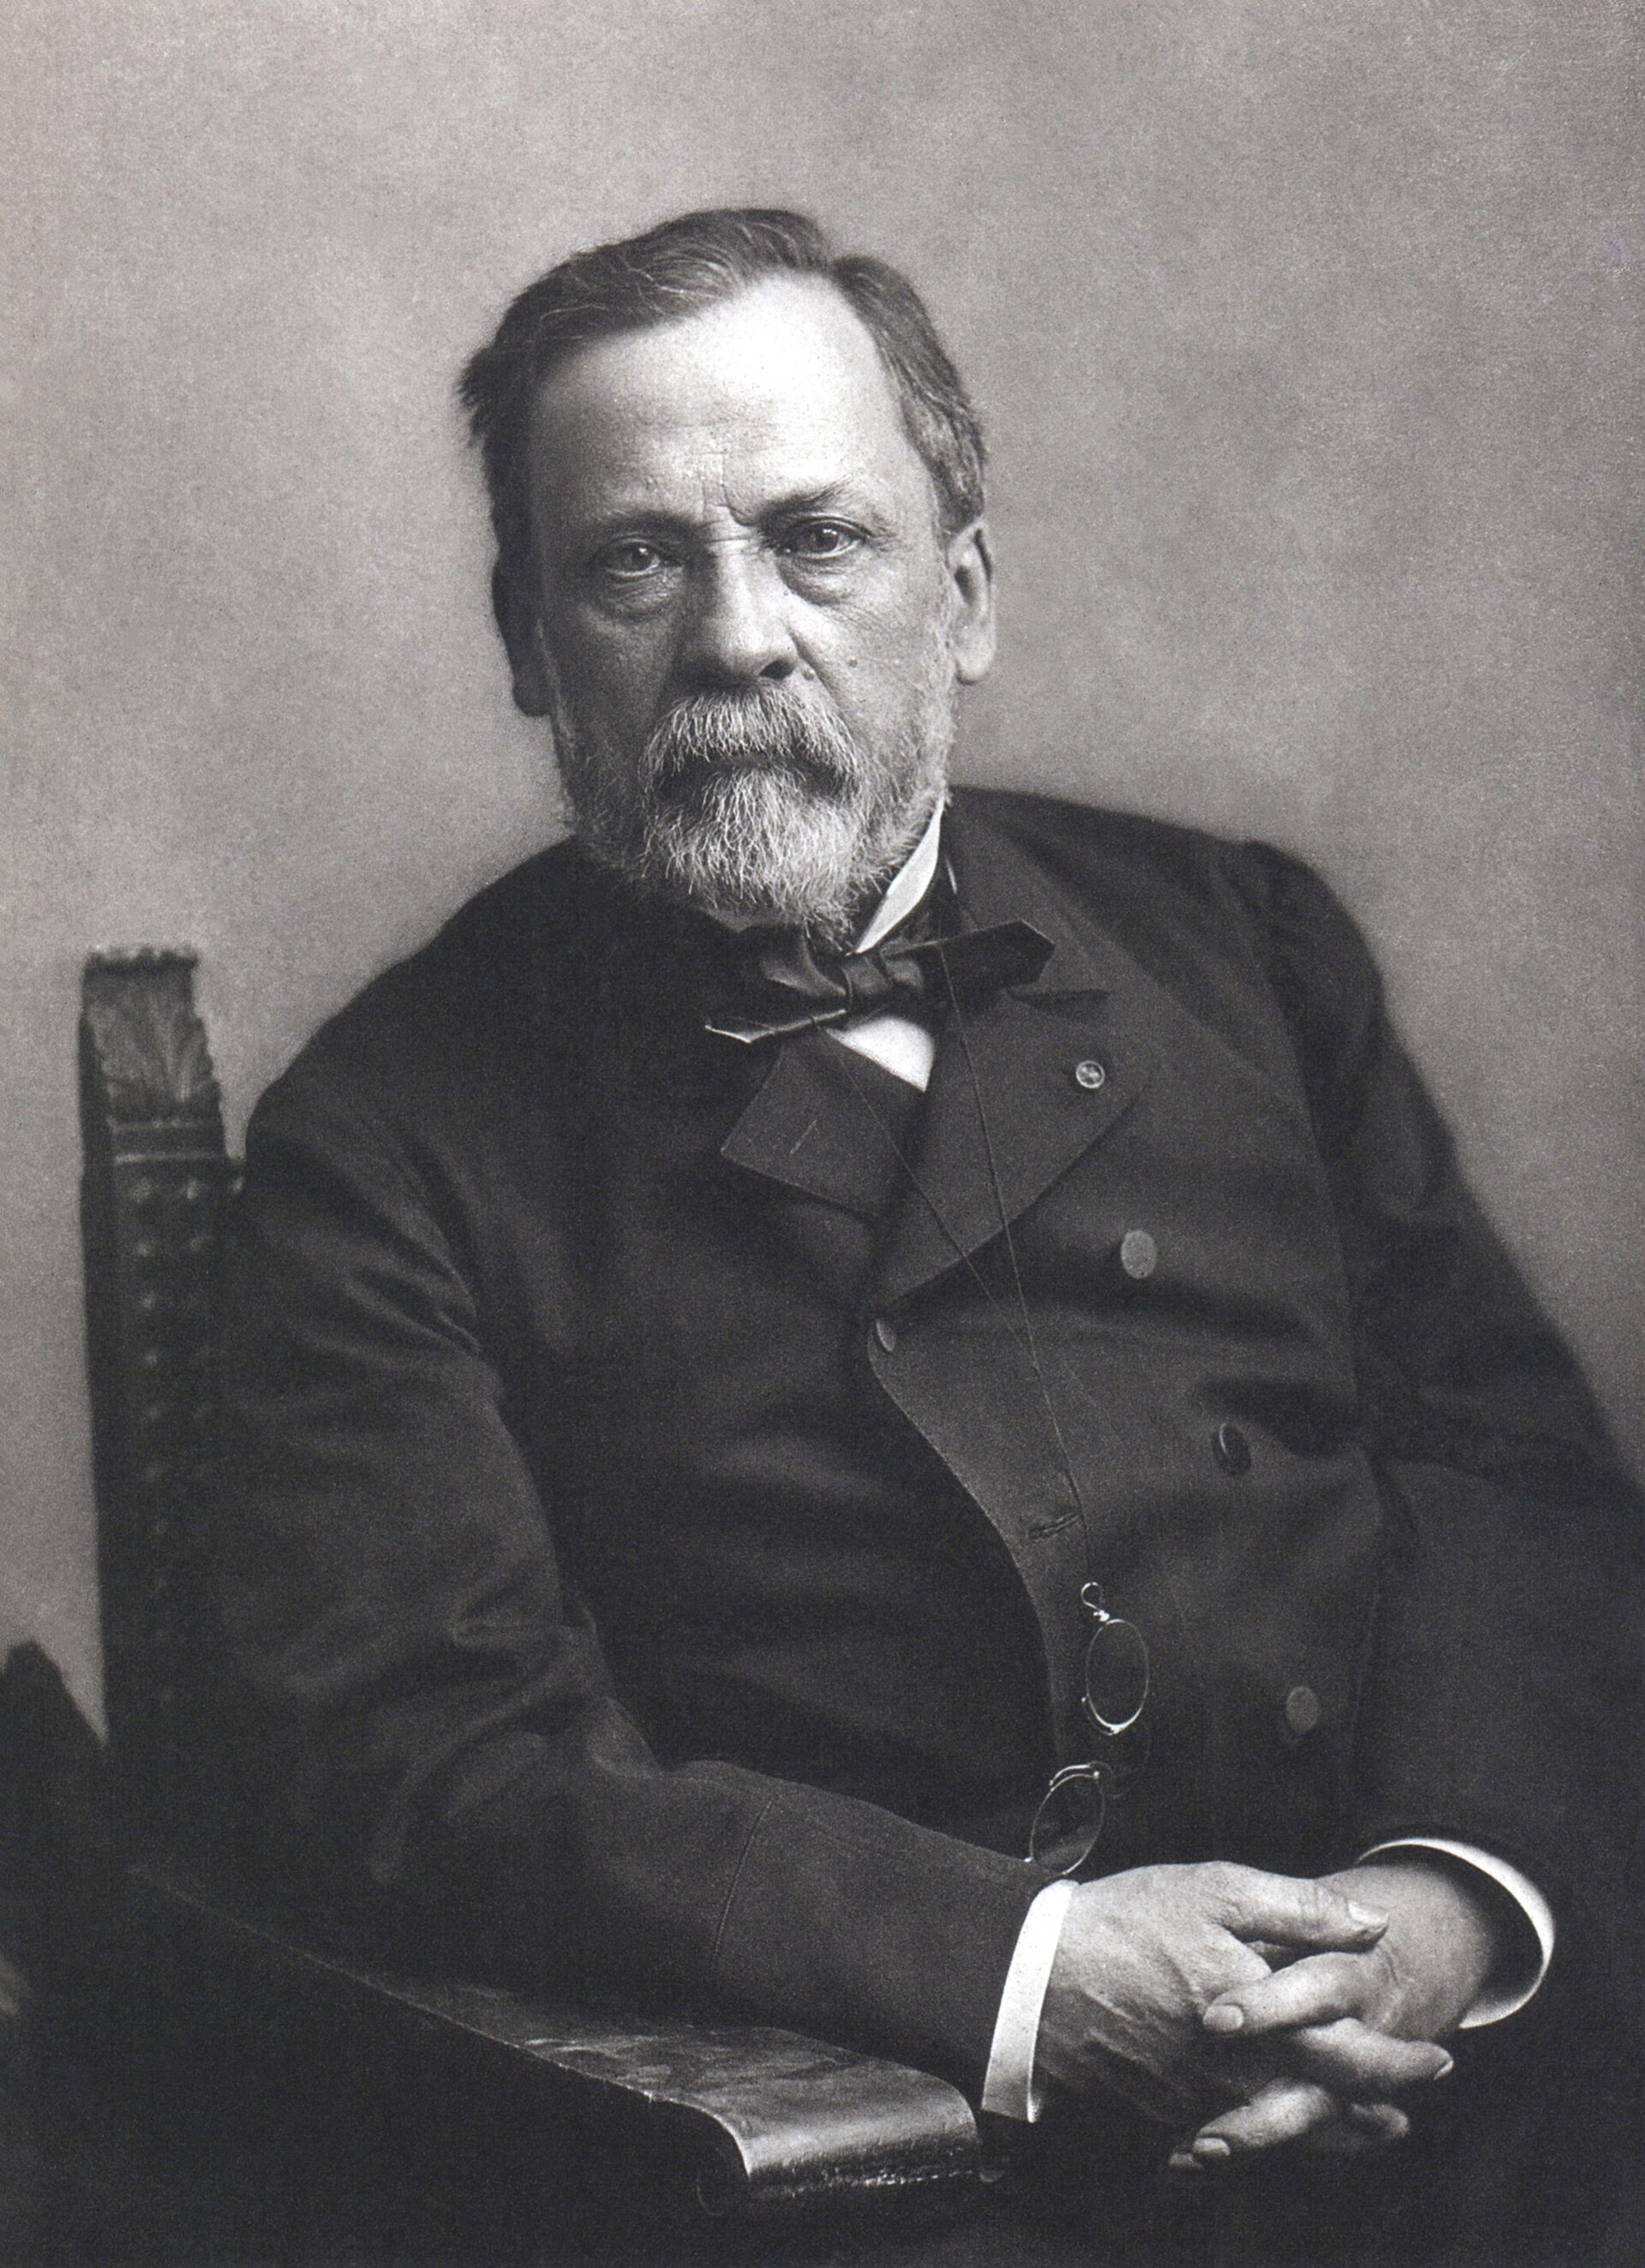
\includegraphics[height=5cm]{images/book1/pasteur.jpg}

{\small Louis Pasteur (1822--1895), photographed by Paul Nadar.}
\end{minipage}\qquad
\begin{minipage}[t]{0.36\linewidth}\centering
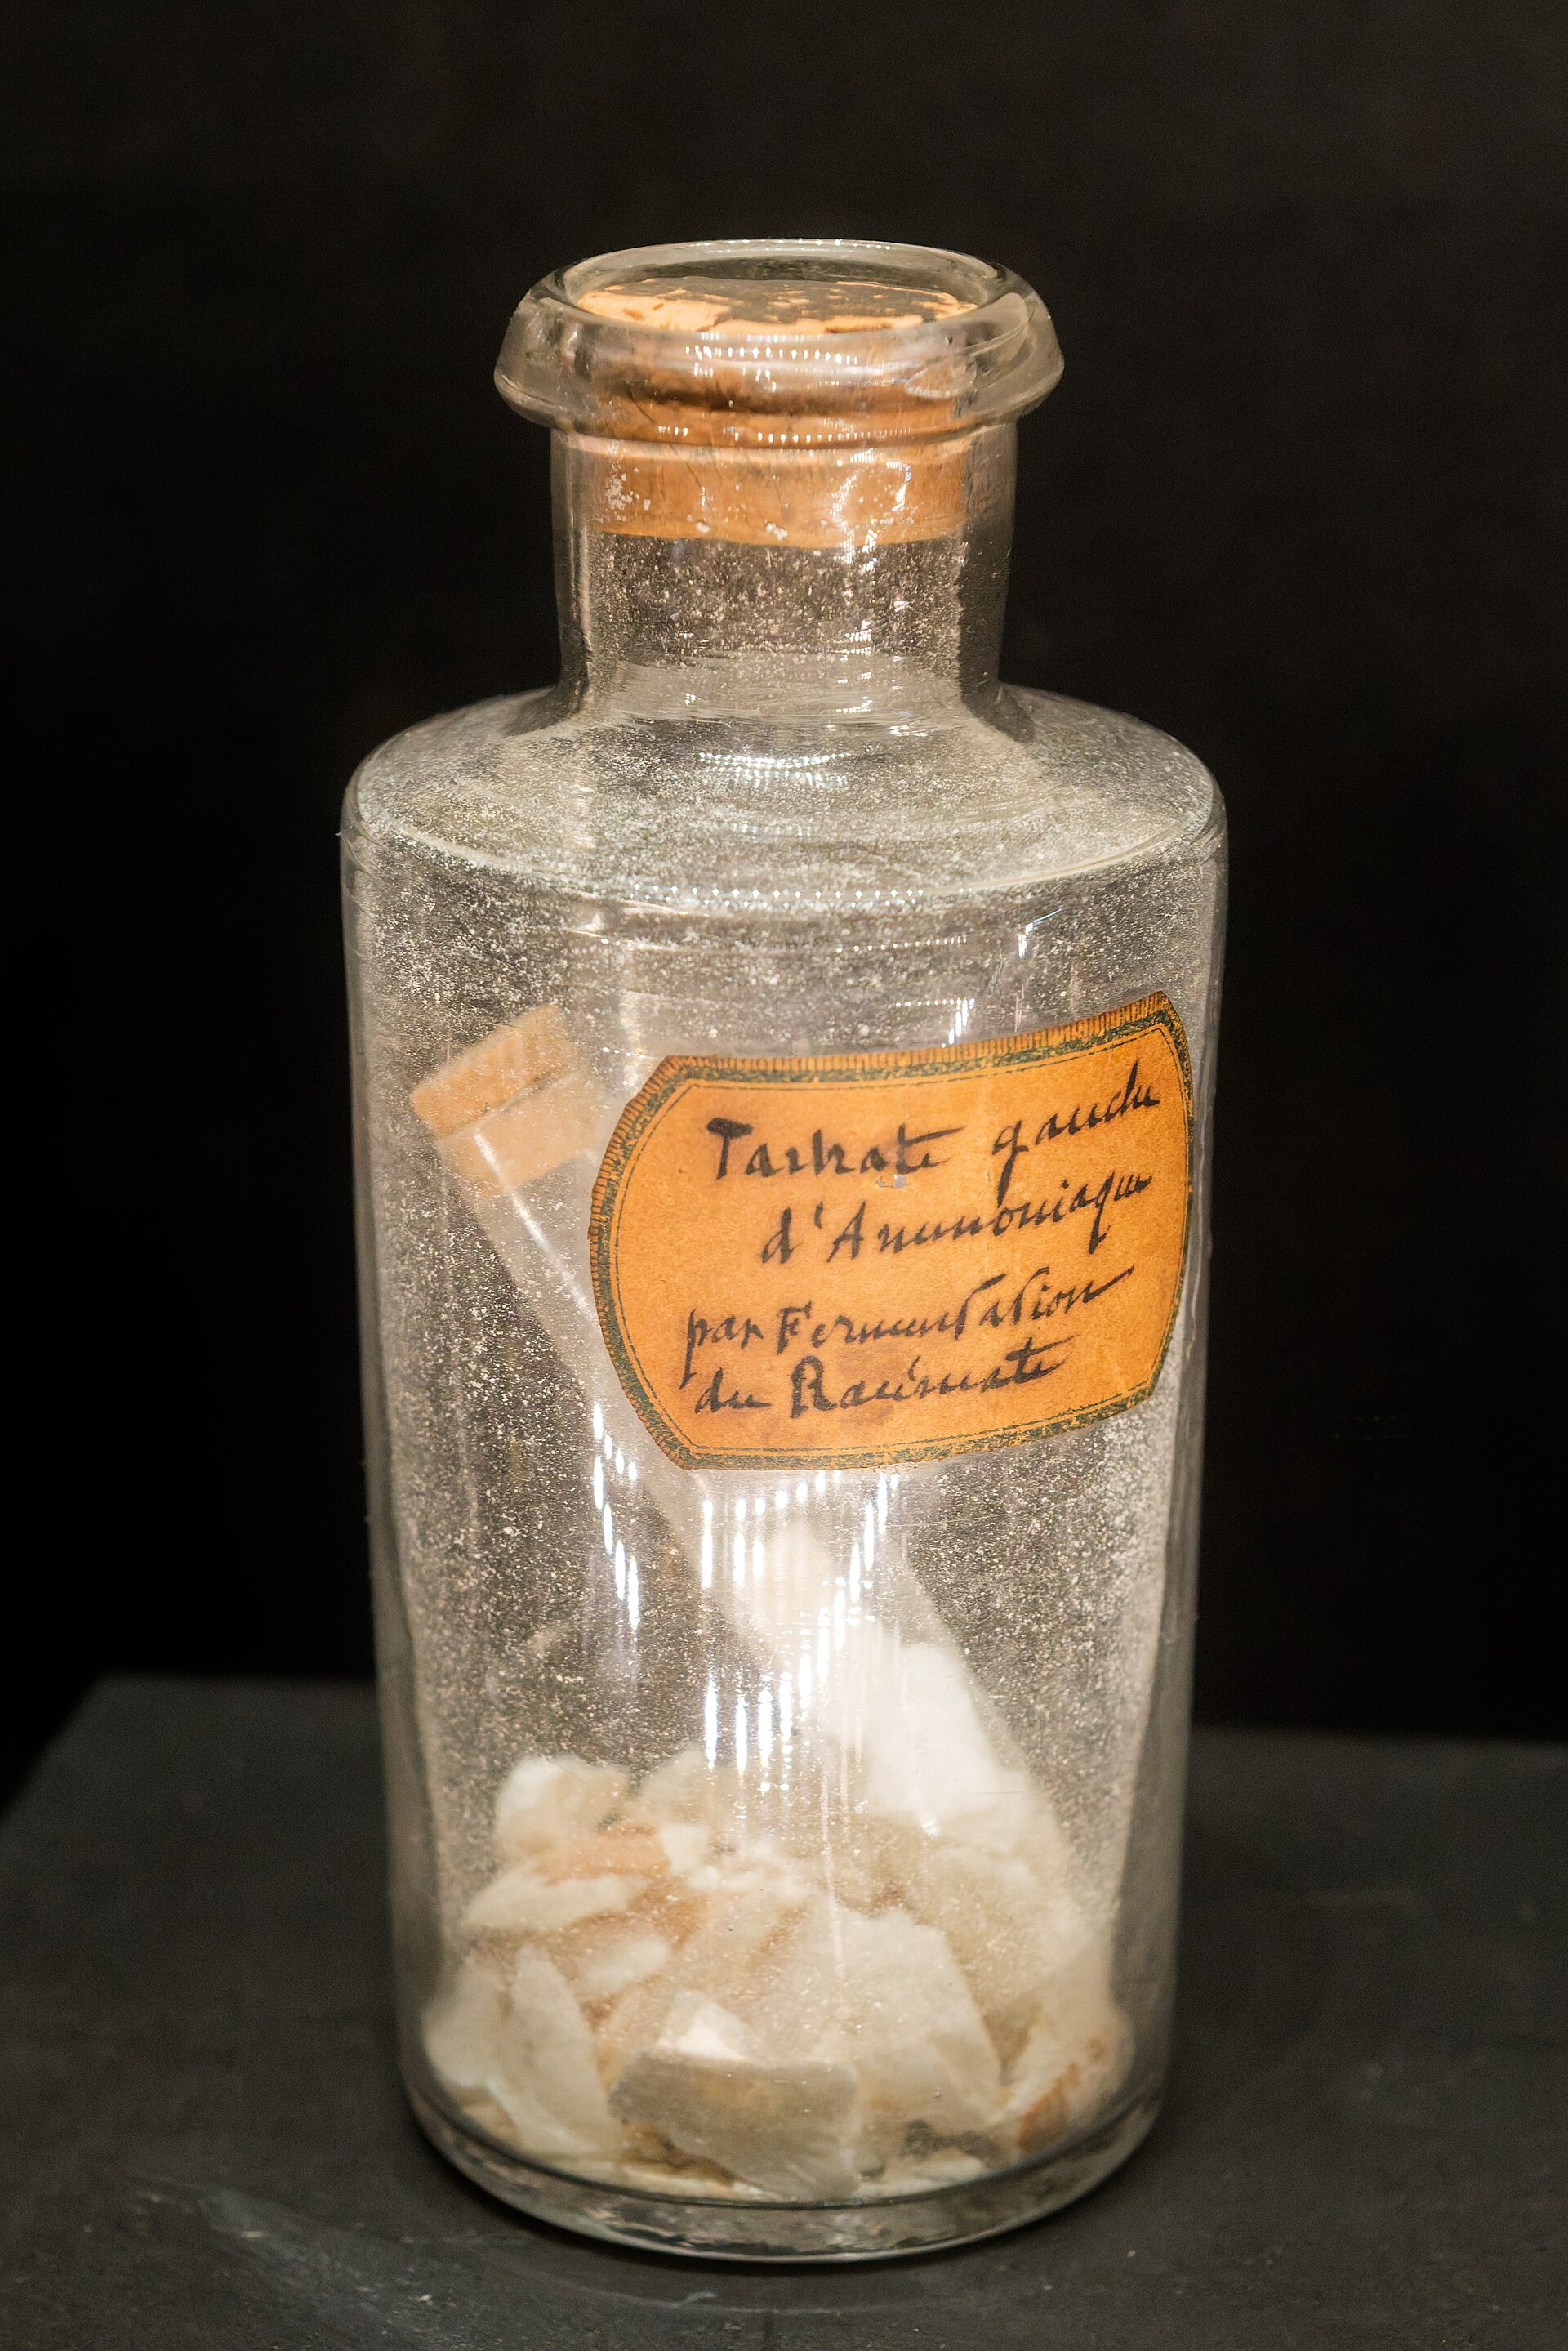
\includegraphics[height=5cm]{images/book1/tartrate-crystals.jpg}

{\small Ammonium tartrate crystals from Pasteur's collection. Photo
Marie-Lan Taÿ Pamart, CC BY 4.0.}
\end{minipage}
\end{omfigure}

\section{Z and E isomers}


\begin{definition}[Z and E isomers]\label{def:g12:stereochemistry:z-e}
When each carbon of a \ce{C=C} \omterm{def:g10:lewis-and-shape:multiple-bond}{double bond} carries two different \omterm{def:g7:atoms-and-molecules:atom}{atoms}
or groups, two \omterm{def:g12:stereochemistry:stereoisomer}{stereoisomers} exist, because the \omterm{def:g10:lewis-and-shape:multiple-bond}{double bond} does not
rotate. On each carbon, the group whose \omterm{def:g7:atoms-and-molecules:atom}{atom} bonded to it has the larger
\omterm{def:g9:inside-the-atom:atomic-number}{atomic number} has priority. If the two priority groups are on the same
side of the \omterm{def:g10:lewis-and-shape:multiple-bond}{double bond}, the isomer is \emph{Z}\index{Z isomer}; if they
are on opposite sides, it is \emph{E}\index{E isomer}.
\end{definition}

\begin{method}[Z or E?]\label{met:g12:stereochemistry:z-e}
\begin{enumerate}
  \item Check that each carbon of the \omterm{def:g10:lewis-and-shape:multiple-bond}{double bond} carries two different
        groups; otherwise there is no \omterm{def:g12:stereochemistry:z-e}{Z}/\omterm{def:g12:stereochemistry:z-e}{E} isomerism.
  \item On each carbon, give priority to the group whose first \omterm{def:g7:atoms-and-molecules:atom}{atom} has
        the larger \omterm{def:g9:inside-the-atom:atomic-number}{atomic number} (the full rules for ties are given in
        the Year 1 volume).
  \item Same side: \omterm{def:g12:stereochemistry:z-e}{Z}. Opposite sides: \omterm{def:g12:stereochemistry:z-e}{E}.
\end{enumerate}
\end{method}

\begin{omfigure}
\setchemfig{atom sep=2em}
\begin{tabular}{cc}
\chemfig{C(-[:150]H_3C)(-[:210]H)=C(-[:30]CH_3)(-[:-30]H)} &
\chemfig{C(-[:150]H_3C)(-[:210]H)=C(-[:30]H)(-[:-30]CH_3)} \\[4pt]
\small (\omterm{def:g12:stereochemistry:z-e}{Z})-but-2-ene: \ce{CH3} groups on the same side &
\small (\omterm{def:g12:stereochemistry:z-e}{E})-but-2-ene: \ce{CH3} groups on opposite sides
\end{tabular}

{\small The two \omterm{def:g12:stereochemistry:stereoisomer}{stereoisomers} of but-2-ene. On each carbon, \ce{CH3}
(carbon, $Z = 6$) has priority over \ce{H} ($Z = 1$). They are
\omterm{def:g12:stereochemistry:diastereomer}{diastereomers}: they boil at different temperatures.}
\end{omfigure}

\section{Conformations}

\begin{definition}[Conformation]\label{def:g12:stereochemistry:conformation}
The \omterm{def:g7:atoms-and-molecules:atom}{atoms} of a \omterm{def:g7:atoms-and-molecules:molecule}{molecule} can rotate about a single bond. Each arrangement
reached by such rotations is a \emph{conformation}\index{conformation} of
the \omterm{def:g7:atoms-and-molecules:molecule}{molecule}. Conformations of one \omterm{def:g7:atoms-and-molecules:molecule}{molecule} are not \omterm{def:g11:organic-skeletons:isomer}{isomers}: they turn
into one another all the time at room temperature.
\end{definition}

\begin{omfigure}
\begin{tikzpicture}[font=\small]
  \pic (s) at (0,0) {omnewman={90}{30}};
  \foreach \k in {1,2,3} { \node at (s-f\k) {H}; \node at (s-b\k) {H}; }
  \node[anchor=north, align=center] at (0,-1.7) {staggered: the H atoms\\ of the two carbons alternate};
  \pic (e) at (5,0) {omnewman={90}{112}};
  \foreach \k in {1,2,3} { \node at (e-f\k) {H}; \node[black!60] at (e-b\k) {H}; }
  \node[anchor=north, align=center] at (5,-1.7) {eclipsed: they face each\\ other (drawn slightly apart)};
\end{tikzpicture}

{\small Two \omterm{def:g12:stereochemistry:conformation}{conformations} of ethane, \ce{CH3-CH3}, seen along the
\ce{C-C} bond: the front carbon is the centre, the back carbon the circle.
The staggered \omterm{def:g12:stereochemistry:conformation}{conformation}, where the \omterm{def:g7:atoms-and-molecules:atom}{atoms} are farthest apart, is the
most stable.}
\end{omfigure}

\begin{remark}[Why it matters]\label{rem:g12:stereochemistry:matters}
Living things are built of \omterm{def:g12:stereochemistry:chiral}{chiral} \omterm{def:g7:atoms-and-molecules:molecule}{molecules} (proteins, sugars), and the
receptors and enzymes made of them distinguish \omterm{def:g12:stereochemistry:enantiomer}{enantiomers}: two
\omterm{def:g12:stereochemistry:enantiomer}{enantiomers} can smell, taste or act as medicines very differently. That
is why chemists who make a drug with an \omterm{def:g12:stereochemistry:chiral}{asymmetric carbon} must know
which enantiomer they make, and test each one.
\end{remark}

\section{Exercises}

\begin{exercise}[$\star$]\label{exo:g12:stereochemistry:1}
Which of these \omterm{def:g7:atoms-and-molecules:molecule}{molecules} have an \omterm{def:g12:stereochemistry:chiral}{asymmetric carbon}? Mark it with a star.
Butan-2-ol \ce{CH3-CH(OH)-CH2-CH3}; propan-2-ol \ce{CH3-CH(OH)-CH3};
2-chlorobutane; lactic acid \ce{CH3-CH(OH)-COOH}.
\end{exercise}

\begin{exercise}[$\star$]\label{exo:g12:stereochemistry:2}
Is each isomer \omterm{def:g12:stereochemistry:z-e}{Z} or \omterm{def:g12:stereochemistry:z-e}{E}?
\begin{center}
\setchemfig{atom sep=1.8em}
\chemfig{C(-[:150]Cl)(-[:210]H)=C(-[:30]Cl)(-[:-30]H)} \qquad
\chemfig{C(-[:150]H_3C)(-[:210]H)=C(-[:30]H)(-[:-30]CH_2-CH_3)}
\end{center}
\end{exercise}

\begin{exercise}[$\star$]\label{exo:g12:stereochemistry:3}
Which are \omterm{def:g12:stereochemistry:chiral}{chiral}: a glove, a spoon, a screw, a cube? Which of the
\omterm{def:g7:atoms-and-molecules:molecule}{molecules} \ce{CH2Cl2} and \ce{CHFClBr} is \omterm{def:g12:stereochemistry:chiral}{chiral}?
\end{exercise}

\begin{exercise}[$\star$]\label{exo:g12:stereochemistry:4}
What is a \omterm{def:g12:stereochemistry:enantiomer}{racemic mixture}? Does it smell of spearmint, of caraway, or of
both, in the case of carvone?
\end{exercise}

\begin{exercise}[$\star$]\label{exo:g12:stereochemistry:5}
Can but-1-ene \ce{CH2=CH-CH2-CH3} exist as \omterm{def:g12:stereochemistry:z-e}{Z} and \omterm{def:g12:stereochemistry:z-e}{E isomers}? Why?
\end{exercise}

\begin{exercise}[$\star\star$]\label{exo:g12:stereochemistry:6}
Draw the two \omterm{def:g12:stereochemistry:enantiomer}{enantiomers} of butan-2-ol in \omterm{def:g12:stereochemistry:cram}{Cram representation}, with a
mirror between them.
\end{exercise}

\begin{exercise}[$\star\star$]\label{exo:g12:stereochemistry:7}
How many \omterm{def:g12:stereochemistry:stereoisomer}{stereoisomers} do these have: 2-chlorobutane;
2,3-dichlorobutane \ce{CH3-CHCl-CHCl-CH3}; pent-2-ene
\ce{CH3-CH=CH-CH2-CH3}?
\end{exercise}

\begin{exercise}[$\star\star$]\label{exo:g12:stereochemistry:8}
Say whether these pairs are \omterm{def:g12:stereochemistry:enantiomer}{enantiomers}, \omterm{def:g12:stereochemistry:diastereomer}{diastereomers} or the same
\omterm{def:g7:atoms-and-molecules:molecule}{molecule}: L- and D-tartaric acid; L- and meso-tartaric acid; (\omterm{def:g12:stereochemistry:z-e}{Z})- and
(\omterm{def:g12:stereochemistry:z-e}{E})-but-2-ene; meso-tartaric acid and its own mirror image.
\end{exercise}

\begin{exercise}[$\star\star$]\label{exo:g12:stereochemistry:9}
Butane, \ce{CH3-CH2-CH2-CH3}, seen along its central bond. Draw the
staggered \omterm{def:g12:stereochemistry:conformation}{conformation} where the two \ce{CH3} groups are opposite, and
an eclipsed one where they face each other. Which is the more stable?
Why?
\end{exercise}

\begin{exercise}[$\star\star$]\label{exo:g12:stereochemistry:10}
meso-Tartaric acid has two \omterm{def:g12:stereochemistry:chiral}{asymmetric carbons} but is not \omterm{def:g12:stereochemistry:chiral}{chiral}.
Explain, using its mirror plane.
\end{exercise}

\begin{exercise}[$\star\star$]\label{exo:g12:stereochemistry:11}
Draw and name the \omterm{def:g12:stereochemistry:z-e}{Z} and \omterm{def:g12:stereochemistry:z-e}{E isomers} of pent-2-ene.
\end{exercise}

\begin{exercise}[$\star\star\star$]\label{exo:g12:stereochemistry:12}
2,3-Dibromobutane \ce{CH3-CHBr-CHBr-CH3} has two \omterm{def:g12:stereochemistry:chiral}{asymmetric carbons}.
Draw its \omterm{def:g12:stereochemistry:stereoisomer}{stereoisomers} in the zigzag representation used for tartaric
acid, and show that one of them is a meso form.
\end{exercise}

\begin{exercise}[$\star\star\star$]\label{exo:g12:stereochemistry:13}
A drug \omterm{def:g7:atoms-and-molecules:molecule}{molecule} has one \omterm{def:g12:stereochemistry:chiral}{asymmetric carbon}. Its \omterm{def:g10:synthesis-yield:synthesis}{synthesis} gives a \omterm{def:g12:stereochemistry:enantiomer}{racemic
mixture}, but only one enantiomer fits the \omterm{def:g12:stereochemistry:chiral}{chiral} receptor it must act
on. What fraction of the racemic medicine is active? Give two ways a
chemist could do better.
\end{exercise}

\begin{exercise}[$\star\star\star$]\label{exo:g12:stereochemistry:14}
Hexa-2,4-diene, \ce{CH3-CH=CH-CH=CH-CH3}, has two \omterm{def:g10:lewis-and-shape:multiple-bond}{double bonds}, each
able to be \omterm{def:g12:stereochemistry:z-e}{Z} or \omterm{def:g12:stereochemistry:z-e}{E}. How many \omterm{def:g12:stereochemistry:stereoisomer}{stereoisomers} does it have? (Beware of the
symmetry of the \omterm{def:g7:atoms-and-molecules:molecule}{molecule}.)
\end{exercise}

\begin{exercise}[$\star\star\star$]\label{exo:g12:stereochemistry:15}
A sugar \omterm{def:g7:atoms-and-molecules:molecule}{molecule} has three \omterm{def:g12:stereochemistry:chiral}{asymmetric carbons} and no symmetry. How many
\omterm{def:g12:stereochemistry:stereoisomer}{stereoisomers} can it have at most? How many pairs of \omterm{def:g12:stereochemistry:enantiomer}{enantiomers} is
that? How many \omterm{def:g12:stereochemistry:diastereomer}{diastereomers} does each stereoisomer have?
\end{exercise}

\section{Problem: Pasteur's Crystals}


\begin{problem}[{Weekend problem --- tartaric acid has two asymmetric
carbons: how many stereoisomers does it really have?}]
\label{pb:g12:stereochemistry:1}
% ledger: mp:tartaric-L, aw:C, aw:H, aw:O
The forms of tartaric acid, \ce{HOOC-CH(OH)-CH(OH)-COOH}, played a
decisive part in the discovery that \omterm{def:g7:atoms-and-molecules:molecule}{molecules} can be handed. L-Tartaric acid melts at about \qty{169}{\celsius}.

\medskip
\noindent\textbf{Part I --- The \omterm{def:g7:atoms-and-molecules:molecule}{molecule}.}
\begin{enumerate}
  \item Give the \omterm{def:g11:organic-skeletons:formulas}{molecular formula} of tartaric acid and its \omterm{def:g10:the-mole:molar-mass}{molar mass}.
  \item Name its \omterm{def:g11:functional-groups:functional-group}{functional groups}, and say how many of each.
  \item Which carbon \omterm{def:g7:atoms-and-molecules:atom}{atoms} are asymmetric? List the four groups of each.
  \item According to the rule of this chapter, how many \omterm{def:g12:stereochemistry:stereoisomer}{stereoisomers}
        could it have at most?
\end{enumerate}

\medskip
\noindent\textbf{Part II --- The \omterm{def:g12:stereochemistry:stereoisomer}{stereoisomers}.}
\begin{enumerate}[resume]
  \item In the zigzag drawing of L-tartaric acid, are the \ce{OH} groups
        drawn with solid or dashed wedges?
  \item Draw its mirror image. Can the two be superimposed? Name the
        mirror image.
  \item Draw the form with one solid and one dashed wedge. Rotate it in
        your mind about the central bond, and find a mirror plane.
  \item Is this form \omterm{def:g12:stereochemistry:chiral}{chiral}? What is it called?
  \item Explain why tartaric acid has only three \omterm{def:g12:stereochemistry:stereoisomer}{stereoisomers}.
  \item Say whether L and D, then L and meso, are \omterm{def:g12:stereochemistry:enantiomer}{enantiomers} or
        \omterm{def:g12:stereochemistry:diastereomer}{diastereomers}.
\end{enumerate}

\medskip
\noindent\textbf{Part III --- Properties.}
\begin{enumerate}[resume]
  \item At what temperature does D-tartaric acid melt? Why?
  \item Must meso-tartaric acid melt at the same temperature? Why?
  \item Carvone shows that two \omterm{def:g12:stereochemistry:enantiomer}{enantiomers} can smell different. Why can
        a nose tell them apart while a thermometer cannot?
  \item A \omterm{def:g12:stereochemistry:enantiomer}{racemic mixture} of L and D tartaric acid: is it a \omterm{def:g6:pure-substances-and-mixtures:pure-substance}{pure
        substance}? Is it optically active as a whole?
\end{enumerate}

\medskip
\noindent\textbf{Part IV --- Pasteur.}
\begin{enumerate}[resume]
  \item Pasteur's racemic salt gave crystals of two mirror-image shapes.
        What did each crystal contain?
  \item From \qty{10.0}{g} of racemic salt, what mass of each kind of
        crystal could he expect?
  \item Why does the meso form never appear among these crystals?
  \item How could he check, after sorting, that the two piles were
        \omterm{def:g12:stereochemistry:enantiomer}{enantiomers}?
  \item 3-Chlorobutan-2-ol, \ce{CH3-CHCl-CH(OH)-CH3}, also has two
        \omterm{def:g12:stereochemistry:chiral}{asymmetric carbons}. How many \omterm{def:g12:stereochemistry:stereoisomer}{stereoisomers} does it have? Why does
        it not lose one like tartaric acid?
  \item State the final answer: how many \omterm{def:g12:stereochemistry:stereoisomer}{stereoisomers} does tartaric acid
        have?
\end{enumerate}
\end{problem}
